%% ==========================================================================
%% OpenThomas -- NeurIPS 2026 workshop version (4-page, RSI-focused).
%% Uses the official NeurIPS style (2025 dropped in; swap in the specific
%% workshop's neurips_2026.sty when the workshop is chosen).
%%
%% Option set here: [preprint] = named, arXiv-ready. For a double-blind
%% workshop use [dblblindworkshop]; single-blind use [sglblindworkshop];
%% camera-ready use [final]. NeurIPS workshop limit is typically 4 pages
%% EXCLUDING references and appendix.
%% ==========================================================================
\documentclass{article}
\usepackage[preprint,nonatbib]{neurips_2025}

\usepackage[utf8]{inputenc}
\usepackage[T1]{fontenc}
\usepackage{amsmath,amssymb}
\usepackage{booktabs}
\usepackage{microtype}
\usepackage{tikz}
\usetikzlibrary{arrows.meta, positioning, calc, fit, backgrounds}
\definecolor{kfill}{RGB}{224,236,247}
\definecolor{kline}{RGB}{70,120,170}
\definecolor{afill}{RGB}{250,224,190}
\definecolor{aline}{RGB}{210,120,30}

\title{Keeping the Judge Off the Edit Surface:\\ Gated Recursive
Self-Improvement on a Strong-Evaluator Domain}

\author{%
  Thomas Wang \\
  \texttt{thomas@openthomas.com} \\
  \texttt{github.com/PredictionMarketTrader/openthomas}
}

\begin{document}
\maketitle

\begin{abstract}
Near-term recursive self-improvement (RSI) is optimization of an agent's
\emph{harness}, and its first bottleneck is evaluator strength. But a strong
evaluator only relocates the danger: an optimizer that can edit its own judge
will lower the bar rather than clear it. We present the self-improvement design
of \textbf{OpenThomas}, an open-source trading agent for weather prediction
markets --- a domain with an unusually strong evaluator (daily, objective NWS
settlement; leak-free replay). Its codebase is split into a \emph{kernel} plane
(promotion gate, parameter bounds, risk rails, truth pipeline) that only the
operator writes, and an \emph{agent} plane (decision parameters, forecast
prompt, strategy code) that an evolution loop writes \emph{only through the
kernel gate}. The split is the security model: the judge is structurally off the
optimizer's edit surface. The gate scores candidates on leak-free replay with
four anti-gaming properties (held-in/held-out splits, totals-not-ratios scoring,
out-of-sample regret rollback, and a calibration veto), and a single accept
mechanism absorbs a growing set of mutation operators. In a leak-free replay
over 968 settled markets, the disciplined production rule turns a naked
model-vs-market loss into a positive expectancy by \emph{selectivity} --- the
same evaluator that gates self-improvement also quantifies where the edge is.
\end{abstract}

\section{Introduction}

Framing near-term recursive self-improvement (RSI) as optimization of the
\emph{harness} --- how an agent plans, acts, remembers, and is evaluated ---
identifies \emph{evaluator strength} as the first bottleneck \cite{harness}. Most
RSI testbeds lack a strong evaluator, so ``improvement'' is measured by a proxy
the optimizer can drift. We start from a domain that supplies an unusually strong
one, and confront the failure mode that a strong evaluator merely relocates: not
a weak judge, but a \emph{gameable} one. An optimizer that can edit its own judge
finds it easier to lower the bar than to clear it.

Our testbed is \textbf{OpenThomas}, an open-source autonomous agent that trades
daily station-temperature markets on Kalshi and Polymarket. These markets settle
every day against an objective public record (the U.S.\ National Weather Service
climatological report for one named station), which makes the evaluator
\emph{dense}, \emph{objective}, and --- with historical as-of forecasts and order
books --- \emph{reproducible in leak-free replay}. The agent embodies a
``harness is the edge'' thesis: every frontier language model given real capital
to trade prediction markets has lost money \cite{predarena}, so OpenThomas
confines the language model to a bounded adjustment and puts selectivity,
calibration, and risk in deterministic code. Here we describe the part that makes
it a self-improving system, and the structural guarantee that keeps
self-improvement honest.

\textbf{Contributions.} (i) A self-improvement architecture whose safety is
\emph{architectural}: a kernel/agent plane split keeps the evaluator off the
optimizer's edit surface, enforced today by code structure and on a roadmap to
OS-level process isolation. (ii) A promotion gate with four anti-gaming
properties on leak-free replay, and a single accept mechanism that absorbs a
growing set of mutation operators (decision parameters and forecast prompts
shipped; workflow, code, and weights on the same gate). (iii) Evidence from the
same evaluator: a leak-free replay ablation in which discipline, not a sharper
model, produces the edge.

\section{Weather markets as a strong-evaluator domain}
\label{sec:weather}

Three properties are exactly what RSI asks for and rarely gets. \textbf{Dense,
objective settlement:} each market resolves against one station's observed daily
extreme, once per day, with no interpretive latitude; a desk on ten U.S.\ cities
sees dozens of ground-truth points per day rather than a few per year.
\textbf{A learnable local edge:} markets settle on a \emph{specific} station, and
global forecast models carry systematic, station-specific biases there (a 90-day
hindcast found Miami consensus $1.8$--$2.1$\,\textdegree F cold, Philadelphia
$+2.3$, LAX $-1$) that are estimable from free public data, offline.
\textbf{Leak-free reproducibility:} historical as-of guidance and historical
order books let a replay present the agent exactly the information it would have
had, and no more --- so a candidate rule, and the whole self-improvement loop, can
be scored without the replay silently cheating.

\section{The structural guarantee: kernel and agent planes}
\label{sec:planes}

Self-improvement is safe only if improvement cannot redefine ``improvement.'' So
the codebase is split into two planes, and the split \emph{is} the security model
(Table~\ref{tab:planes}). The \textbf{kernel} plane --- the promotion gate,
parameter bounds, the risk engine and all safety rails, the truth pipeline, and
the journal schema --- is written only by the operator; the evolution loop has no
write path to it. The \textbf{agent} plane --- decision-rule parameters, the
forecast prompt template, and (on the roadmap) workflow structure, strategy code,
and the evolver itself --- is written by the evolution loop, but only
\emph{through} the kernel gate.

\begin{table}[t]
\centering
\small
\begin{tabular}{@{}p{1.5cm}p{8.4cm}p{2.4cm}@{}}
\toprule
\textbf{Plane} & \textbf{Contents} & \textbf{Written by} \\
\midrule
kernel & promotion gate, parameter bounds, risk engine \& safety rails (sizing, exposure caps, kill-switch), truth pipeline, journal schema & operator only \\
agent & decision-rule parameters, forecast prompt template; later: workflow structure, strategy code, the evolver itself & evolution loop, \emph{via the gate} \\
\bottomrule
\end{tabular}
\caption{The plane split is the security model. One line is drawn precisely:
entry-\emph{selectivity} knobs (minimum edge, market-prior blend weight) are
genome parameters under kernel bounds, while sizing, exposure caps, and the
kill-switch are safety rails that can never enter the parameter space --- a kernel
policy test fails any change that tries to move one there.}
\label{tab:planes}
\end{table}

The operator is moved \emph{up} the stack: they set bounds and review lineage,
and are forbidden from hand-tuning trading parameters --- that is what the
evolution loop is for. Today the split is enforced by code structure (the LLM
proposer only ever returns JSON; every file write happens in deterministic code
after the gate has ruled). The deployment roadmap makes it structural in the OS:
kernel paths owned by the operator's user, the evolver running as a user with
write access only to the agent plane, gate decisions crossing a process boundary,
and every promotion an auditable commit authored by the loop itself.

\section{The evolution loop and its gate}
\label{sec:loop}

\begin{figure}[t]
\centering
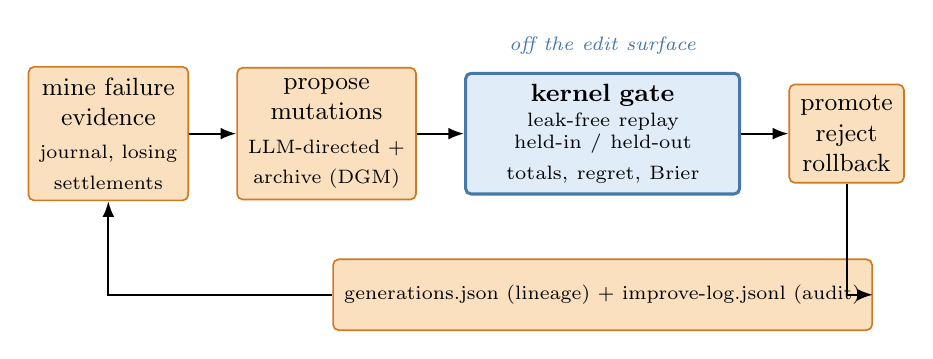
\begin{tikzpicture}[
  font=\small,
  box/.style={draw, rounded corners=2pt, align=center, inner sep=4pt,
              line width=0.6pt, minimum height=9mm},
  a/.style={box, fill=afill, draw=aline},
  k/.style={box, fill=kfill, draw=kline, line width=1.1pt},
  flow/.style={-{Latex[length=2mm]}, line width=0.7pt},
  node distance=6mm,
]
\node[a] (ev) {mine failure\\evidence\\[1pt]\scriptsize journal, losing\\\scriptsize settlements};
\node[a, right=of ev] (prop) {propose\\mutations\\[1pt]\scriptsize LLM-directed +\\\scriptsize archive (DGM)};
\node[k, right=of prop, text width=32mm] (gate) {\textbf{kernel gate}\\[1pt]\scriptsize leak-free replay\\\scriptsize held-in / held-out\\\scriptsize totals, regret, Brier};
\node[a, right=of gate] (out) {promote\\reject\\rollback};
\node[a, below=8mm of gate] (lin) {\scriptsize generations.json (lineage) + improve-log.jsonl (audit)};

\draw[flow] (ev) -- (prop);
\draw[flow] (prop) -- (gate);
\draw[flow] (gate) -- (out);
\draw[flow] (out) |- (lin);
\draw[flow] (lin) -| (ev);
\node[kline, font=\scriptsize\itshape, above=1mm of gate] {off the edit surface};
\end{tikzpicture}
\caption{The evolution loop: propose--evaluate--accept with a Darwin G\"odel
Machine-style archive of past variants as mutation parents. The gate (kernel,
shaded) is the only path to the agent plane and is never on the optimizer's edit
surface. Rejected and rolled-back generations stay on file as future parents.}
\label{fig:loop}
\end{figure}

Three loops nest (Figure~\ref{fig:loop}). A fast \emph{trading} loop runs the
champion parameters and never waits on the others. A \emph{reflection} loop
distills settled trades into bounded playbook rules. The \emph{evolution} loop
mines failure evidence, proposes mutations --- LLM-directed by the evidence, plus
Gaussian mutations from an \emph{archive} of past variants (Darwin G\"odel
Machine-style \cite{dgm}, against diversity collapse) --- and submits them to the
gate.

\textbf{The gate (kernel, frozen)} scores a candidate \emph{strategy callable} on
leak-free replay with four anti-gaming properties. \emph{Held-in/held-out:}
winners are picked on older days; the freshest settled days only get a veto, and
the window rolls forward daily, so repeated meta-cycles face new data rather than
re-fitting one static split. \emph{Totals-not-ratios:} scoring is total replay
PnL with a minimum trade count --- a rule that trades twice cannot win on ratio, a
rule that trades nothing cannot win on drawdown. \emph{Out-of-sample regret
rollback:} each cycle first re-scores the active generation against its parent on
the fresh window and reverts if the parent now wins --- an overfit promotion is
undone before anything new is proposed. \emph{Calibration veto:} for the forecast
operator, a prompt that wins PnL while worsening Brier got lucky, and luck does
not promote. Generation~0 is the operator's config and applies no overrides.

\textbf{One gate, growing write surface.} Improvement axes are unified as mutation
operators feeding the \emph{same} accept mechanism: playbook rules and
calibration refits (shipped), decision-parameter and forecast-prompt mutation
(shipped), then workflow structure, then agent-plane code diffs (which add shadow
paper-trading and human diff review), then LoRA/GRPO weight updates with a
time-discounted reward $R\cdot e^{-\lambda\,\text{days-to-close}}$ --- a trained
adapter is just another candidate at the same gate. The admission rule is strict:
a parameter enters the space only when the gate can actually discriminate on it.
\emph{Tuning what you cannot measure is drift, not improvement.} This is why code
diffs come last (they need the strongest evaluation: replay \emph{plus} shadow
trading \emph{plus} human review), and why the enterprise is anchored to a
strong-evaluator domain in the first place.

\section{Evidence from the same evaluator}
\label{sec:results}

The gate's trustworthiness rests on one discipline: \emph{never let the replayed
market know something the replayed model does not.} Station bias/$\sigma$ are
learned strictly before the replay window; prices come from snapshot candlesticks
that precede the temperature extreme being bet on (a single timing leak once
turned a losing rule into a fake winner; fixing it turned it back). The same
leak-free pipeline that scores candidate generations also lets us quantify where
the edge is (Table~\ref{tab:ablation}): over 968 settled markets, a naked
model-vs-market rule barely loses, but blending the model with the market prior
more than halves activity ($425\!\to\!184$ trades) and flips expectancy positive.
Selectivity, not a sharper model, is the edge --- the harness thesis, measured by
the same judge that governs self-improvement.

\begin{table}[t]
\centering
\small
\begin{tabular}{@{}p{5.6cm}rrr@{}}
\toprule
\textbf{Decision rule (leak-free replay, fees in)} & \textbf{Trades} & \textbf{Win} & \textbf{PnL/ct} \\
\midrule
Naked model-vs-market & 425 & 41\% & $-\$0.007$ \\
\quad $+$ learned station bias & 396 & 39\% & $-\$0.005$ \\
\quad\quad $+$ market-prior blend (production) & 184 & 45\% & $+\$0.028$ \\
\bottomrule
\end{tabular}
\caption{Replay over 968 settled markets (2026-06-24 to 07-14; timing-safe
snapshots; bias learned out-of-window). The market-prior blend more than halves
activity and flips expectancy positive: \emph{selectivity} is the edge. Small
sample, paper mode --- an existence proof, not a track record.}
\label{tab:ablation}
\end{table}

\section{Failure modes and limitations}

Each classic RSI failure mode has a structural counter here. \emph{Reward hacking}
$\to$ the judge (gate, truth pipeline, risk engine) is off the edit surface, with
hard bounds and totals-not-ratios scoring. \emph{Overfitting the evaluator} $\to$
rolling held-out veto plus regret rollback on post-promotion data.
\emph{Diversity collapse} $\to$ archive-parent random mutations alongside
LLM-directed ones. \emph{Weak evaluator} $\to$ the domain choice itself; operators
without replay data get ``insufficient data,'' not a silent promotion.
\emph{Runaway autonomy} $\to$ the drawdown kill-switch, paper-by-default, and
live-mode two-step opt-in are all kernel and cannot be loosened by the loop; a
dead LLM endpoint degrades evolution to random mutations, and a dead evolution
loop degrades OpenThomas to a static (still disciplined) trader.

Limitations are real. Replay omits the news brief, intraday observations, and the
calibration layer; it measures the template's skill at adjusting the statistical
baseline, the dominant live pathway for weather markets, not the whole live agent.
The results are small-sample and paper-mode --- an existence proof about where the
edge comes from, not a track record; the reference agent's live run is the ongoing
public test. And the strong-evaluator property that makes this domain tractable is
what most other markets lack; extending the gate to weaker-evaluator settings
(via archived-input trace replay) is future work. The system and its live feed are
public.

\small
\begin{thebibliography}{9}
\bibitem{harness} L.~Weng. Harness Engineering for Self-Improvement. Blog post,
2026.
\bibitem{predarena} Prediction Arena: evaluating frontier language models as
autonomous prediction-market traders. arXiv:2604.07355, 2026.
\bibitem{dgm} The Darwin G\"odel Machine: open-ended self-improvement with a
variant archive. 2025.
\end{thebibliography}

\end{document}
